%%%%%%%%%%%%%%%%%%%%%%%%%%%%%%%%%%%%%%%%%%%%%%%%%%%%%%%%%%%%%%%%%%%%%%%
% $Id: header.tex 1229 2009-10-23 13:58:42Z inf6254 $
% This tex document was created by Bj�rn Peem�ller and Stefan Roggensack
%%%%%%%%%%%%%%%%%%%%%%%%%%%%%%%%%%%%%%%%%%%%%%%%%%%%%%%%%%%%%%%%%%%%%%%
\documentclass
  [ twoside            % beidseitiger Druck
  , BCOR=10mm          % Bindekorrektur
  , openright          % Kapitel beginnen auf einer rechten Seite
  , listof=totoc       % Verzeichnisse im Inhaltsverzeichnis
  , bibliography=totoc % Literaturverzeichnis im Inhaltsverzeichnis
  , parskip=half       % Absätze durch einen vergrößerten Zeilenabstand getrennt
%  , draft              % Entwurfsversion
  ]{scrreprt}          % Dokumentenklasse: KOMA-Script Buch

\usepackage{scrhack}

%%%%%%%%%%%%%%%%%%%%%%%%%%%%%%%%%%%%%%%%%%%%%%%%%%%%%%%%%%%%%%%%%%%%%%%
% Packages
%%%%%%%%%%%%%%%%%%%%%%%%%%%%%%%%%%%%%%%%%%%%%%%%%%%%%%%%%%%%%%%%%%%%%%% 
\usepackage{ifpdf}
\ifpdf
  \usepackage{ae}               % Fonts für pdfLaTeX, falls keine cm-super-Fonts installiert
  \usepackage{microtype}        % optischer Randausgleich, falls pdflatex verwandt
  \usepackage[pdftex]{graphicx} % Grafiken in pdfLaTeX
\else
  \usepackage[dvips]{graphicx}  % Grafiken und normales LaTeX
\fi

\usepackage[latin1]{inputenc}         % Input encoding (allow direct use of special characters like "ä")
\usepackage[german]{babel}
\usepackage[T1]{fontenc}
\usepackage[automark]{scrpage2} 	% Schickerer Satzspiegel mit KOMA-Script
\usepackage{setspace}           	% Allow the modification of the space between lines
\usepackage{booktabs}           	% Netteres Tabellenlayout
\usepackage{multicol}               % Mehrspaltige Bereiche
\usepackage{quotchap}               % Beautiful chapter decoration
\usepackage[printonlyused]{acronym} % list of acronyms and abbreviations
\usepackage{subfig}                 % allow sub figures
\usepackage{tabularx}              % Tabellen mit fester Breite

% Layout
\pagestyle{scrheadings}
%\pagestyle{empty}
\clubpenalty = 10000
\widowpenalty = 10000
\displaywidowpenalty = 10000

\makeatletter
\renewcommand{\fps@figure}{htbp}
\makeatother

%% Document properties %%%%%%%%%%%%%%%%%%%%%%%%%%%%%%%%%%%%%%%%%%%%%%%%
\newcommand{\projname}{Edgeblend}
\newcommand{\titel}{Edgeblend}
\newcommand{\subtitel}{Horizontales und vertikales edgeblending f�r Multi-Beamer Systeme}
\newcommand{\Datum}{10. Mai 2010}
\newcommand{\Author}{Markus Knofe and Alexander Treptow}

\ifpdf
  \usepackage{hyperref}
  \definecolor{darkblue}{rgb}{0,0,.5}
  \hypersetup
  	{ colorlinks=true
  	, breaklinks=true
    , linkcolor=darkblue
    , menucolor=darkblue
    , urlcolor=darkblue
    , pdftitle={\projname -- \subtitel}
    , pdfsubject={Master's Thesis}
    , pdfauthor={\Author}
    }
\else
\fi

%% Listings %%%%%%%%%%%%%%%%%%%%%%%%%%%%%%%%%%%%%%%%%%%%%%%%%%%%%%%%%
\usepackage{listings}
\KOMAoptions{listof=totoc} % necessary because of scrhack
\renewcommand{\lstlistlistingname}{List of Listings}
\lstset
  { basicstyle=\small\ttfamily
  , breaklines=true
  , captionpos=b
  , showstringspaces=false
  , keywordstyle={}
  }

\lstnewenvironment{inlinec}
{\spacing{1}\lstset{language=C,nolol,aboveskip=\bigskipamount}}
{\endspacing}

\lstnewenvironment{inlinexml}
{\spacing{1}\lstset{language=XML,nolol,aboveskip=\bigskipamount}}
{\endspacing}

\lstnewenvironment{inlineshell}
{\spacing{1}\lstset{language=sh,nolol,aboveskip=\bigskipamount}}
{\endspacing}

\newcommand{\cinput}[2][]{
  \begin{spacing}{1}
  \lstinputlisting[language=C,nolol,aboveskip=\bigskipamount,#1]{#2}
  \end{spacing}
}

\newcommand{\ccode}[2][]{\mylisting[#1,language=C]{#2}}

\newcommand{\xmlcode}[2][]{\mylisting[#1,language=XML]{#2}}

\newcommand{\mylisting}[2][]{
\begin{spacing}{1}
\lstinputlisting[frame=lines,aboveskip=2\bigskipamount,#1]{#2}
\end{spacing}
}

%% additional commands
\newcommand{\todo}[1]{\marginpar{\textbf{TODO}} \textcolor{red}{#1}}
\newcommand{\code}[1]{\texttt{#1}}

\begin{document}

% \frontmatter
\pagenumbering{Roman}
%%%%%%%%%%%%%%%%%%%%%%%%%%%%%%%%%%%%%%%%%%%%%%%%%%%%%%%%%%%%%%%%%%%%%%%
% Titelseite
\titlehead{
  \centering
  
\includegraphics[width=.5\textwidth]{gfx/fhw}\\
  \bigskip
  \textsc{\Large Fachrichtung Informatik}
}

\subject{Virtual Reality 2 - Projekt}
\title{\titel}
\subtitle{\Large \subtitel}
\date{\vspace{-1cm}{\small Eingereicht am:}\\\smallskip\Datum}
    
\author{}
\publishers{\vfill
  \normalsize
  \begin{minipage}{13cm}

    \bigskip

    \centering
    {\small Eingereicht von:}
    
    \begin{multicols}{2}
      \raggedright
       {\Large B.\,Sc. Markus Knofe}\\
       stra�e nr\\
       2xxxx Hamburg, Deutschland\\
       Tel: +49~(40)~00\,00\,00\\
       E-Mail: markus@knofe.net\\
       MatrNr.: 6718

      \raggedleft
       {\Large B.\,Sc. Alexander Treptow}\\
       Tannenallee 43\\
       22844 Norderstedt, Germany\\
       Tel.: +49~(40)~522\,57\,51\\
       E-Mail: alextreptow@gmx.de\\
       MatrNr.: 6688
    
    \end{multicols}
    
    \bigskip
    \bigskip
    
    {\small Betreut von:}
    \begin{multicols}{2}
      \raggedright
      {\Large Dipl. Medieninf. Martin Egge}\\
      Fachhochschule Wedel\\
      Feldstra�e 143\\
      22880 Wedel, Deutschland\\
      Tel.: +49~(41\,03)~80\,48-810\\
      E-Mail: eg@fh-wedel.de\\
         
      \raggedleft
      {\Large B.\,Sc. Matthias Woggon}\\
      Fachhochschule Wedel\\
      Feldstra�e 143\\
      22880 Wedel, Deutschland\\
      Tel.: +49~(41\,03)~80\,48-49\\
      E-Mail: mwoggon@eyefactive.com\\
    \end{multicols}
 \end{minipage}
}

%\uppertitleback{
%  {\huge \titel}\bigskip\\  
%  {\Large \subtitel}\bigskip\\
%  {\large Pojektbericht von \Author}
  %\begin{abstract}
Nowadays interactive web applications become a growing part in every day life. There is a huge variety of frameworks for supporting development of such web applications. The Hawk framework is written in the non-strict pure functional programming language Haskell, which offers an expressive syntax and an extended type system. So it's ideal for creation of interactive web applications. This thesis will give an example architecture for a real world web application using Hawk framework as well as an abstraction layer for the search engine framework Holumbus to uncouple web application from search engine. Therefore the search web application Hayoo! API Search is reimplemented using Hawk framework, the abstraction layer is worked out and Hawk is extended within the specifications.

%hauptbestandteil dieser arbeit ist das vorgeben einer beispielarchitektur f�r real world web applikationen, in der strikten funktionalen programmiersprache haskell und mit dem web framwork Hawk, sowie einer abstraktionsschicht f�r das suchmaschinen framework holumbus f�r web applikationen um die eigentliche web applikation von der suchmaschine zu entkoppeln. daf�r wird im rahmen dieser arbeit die applikation hayoo! api search mit hawk reimplementiert, der abstaktionslayer erarbeitet und hawk im rahmen der vorgaben erweitert.

\end{abstract}
%}

%\lowertitleback{
%
\includegraphics[width=2.5cm]{gfx/by-nc-sa}\bigskip\\
%Copyright {\small \copyright} 2010 \Author\bigskip\\
%This work is licensed under the Creative Commons Attribution-Noncommercial-Share Alike 3.0 Germany License. To view a copy of this license, visit \url{http://creativecommons.org/licenses/by-nc-sa/3.0/de/} or send a letter to Creative Commons, 171 2nd Street, Suite 300, San Francisco, California, 94105, USA.\bigskip\\
%The template \cite{ThesisTpl} of Bj�rn Peem�ller and Stefan Roggensack was used for the layout.
%}

\maketitle
\tableofcontents
%\listoffigures
%\lstlistoflistings
\cleardoublepage
%\addchap{List of Abbreviations}
% Caution: Keeps the ordering, so please order it yourself!
\begin{acronym}[XXXX]
%\acro{ACID}{Atomicity, Consistency, Isolation, Durability}
\acro{ACP}{Administrator Control Panel}
\acro{AJAX}{Asynchronous JavaScript and XML}
\acro{API}{Application Programming Interface}
\acro{CA}{Certification Authority}
\acro{CAPTCHA}{Completely Automated Public Turing test to tell Computers and Humans Apart}
\acro{CPU}{Central Processing Unit}
\acro{CSS}{Cascading Style Sheets}
\acro{CSV}{Comma Separated Values}
\acro{DB}{Database}
\acro{DOM}{Document Object Model}
\acro{GHC}{Glasgow Haskell Compiler}
\acro{GWT}{Google Web Toolkit}
\acro{Hawk}{Haskell Web Application Kit}
\acro{Hayoo}{Hayoo! API Search}
\acro{HTML}{Hypertext Markup Language}
\acro{HTTP}{Hypertext Transfer Protocol}
\acro{HTTPS}{HTTP Secure}
\acro{HXT}{Haskell XML Toolbox}
\acro{ID}{Identifier}
\acro{IO}{Input and Output}
\acro{JSON}{JavaScript Object Notation}
\acro{MD5}{Message Digest algorithm 5}
\acro{MVC}{Model-View-Controller Pattern}
\acro{PKI}{Public Key Infrastructure}
\acro{SQL}{Structured Query Language}
\acro{SNI}{Server Name Identification}
\acro{SSL}{Secure Socket Layer}
\acro{SSO}{Single Sign-On}
\acro{TLS}{Transport Layer Security}
\acro{URL}{Uniform Resource Locator}
\acro{XHR}{XMLHttpRequest}
\acro{XHTML}{eXtensible Hypertext Markup Language}
\acro{XML}{eXtensible Markup Language}
\acro{XSLT}{Extensible Stylesheet Language Tranformation}
\acro{}{}
%\acro{AST} {Abstract Syntax Tree}
%\acro{CGI} {Common Gateway Interface}
%\acro{CRUD}{Create, Read, Update, Delete}
%\acro{ERM} {Entity-Relationship Model}
%\acro{GHC} {Glasgow Haskell Compiler}
%\acro{HDBC}{Haskell Database Connectivity}
%\acro{HSP} {Haskell Server Pages}
%\acro{HTTP}{Hypertext Transfer Protocol}
%\acro{HXT} {Haskell XML Toolbox}
%\acro{JSON}{JavaScript Object Notation}
%\acro{JVM} {Java Virtual Machine}
%\acro{MVC} {Model, View, Controller}
%\acro{ORM} {Object-Relational Mapping}
%\acro{SQL} {Structured Query Language}
%\acro{URL} {Unified Resource Locator}
%\acro{XML} {Extensible Markup Language}
\end{acronym}
\cleardoublepage

% \mainmatter
\pagenumbering{arabic}
\onehalfspacing
% Chapters
%%%%%%%%%%%%%%%%%%%%%%%%%%%%%%%%%%%%%%%%%%%%%%%%%%%%%%%%%%%%%%%%%%%%%%%
\chapter{Allgemeine Problemstellung}
\label{cha:problemstellung}

%In diesem Teil der Dokumentation soll die Problematik, die der Programmentwicklung zugrunde liegt, dargestellt werden, und zwar unabh�ngig von der programmtechnischen Realisierung. Auch soll aufgef�hrt werden, welche Teile des Problems durch das Programm abgedeckt werden. Bei Seminaraufgaben ist dieser Teil durch die Aufgabenstellung vorgegeben. 
Dieses Kapitel beschreibt den Hintergrund dieser Proektarbeit, umrei�t kurz die Idee hinter dem Projekt und geht auf die Anforderungen ein.

% allgemeine problemstellung
\section{Hintergrund}
Verst�rkte Immersion wird in der Virtual Reality (VR) oft durch gr��ere oder mehrere Projektionsfl�chen erzeugt, so dass der Betrachter den Bezug zu der realen Umgebung verliert. Diese Fl�chen ben�tigen leider meist mehrere Beamer um sie in einer akzeptablen Aufl�sung zu bestrahlen. Es ist nahezu unm�glich die Beamer so im Verh�ltnis zur Fl�che zu positionieren, dass die beleuchteten Stellen auf der Projektionsfl�che sich nicht �berschneiden.

Aus dieser �berschneidung ergeben sich zwei Haupts�chliche Probleme. Zum Einen wird der Bereich der �berschneidung mit doppelter Intensit�t beleuchtet, dies ist extrem auff�llig. Zum Anderen kennt die Rendering-Pipeline die Gr��e der �berlappung nicht, wodurch z.B. Teile eines Objektes �bereinander liegen, die nebeneinander liegen sollten. Sehr Auff�llig ist dies bei interaktiven Anwendungen, wenn die virtuelle Hand (in Form eines Cursors oder �hnlichem) betroffen ist.

Auf den in der FH-Wedel vorhandenen Cave trifft dieses Problem nicht zu, da hier nur ein Beamer zur Zeit je eine Projektionsfl�che bestrahlt. Allerdings bei Anwendungen wie der CoBench, die sehr stark auf Interaktivit�t setzt und zwei Beamer f�r eine Fl�che ben�tigt treten die Probleme auf. In verst�rkter Form treten die Probleme bei sph�rischen Projektionen mit mehreren Beamern auf, da hier die �berlappungen selbst mit komplexen Linsensystemen nur unter gr��tem Aufwand gering gehalten werden k�nnen.

\section{Projektidee}
Im Rahmen dieses Projektes soll daher ein Plug-In entstehen, welches �berschneidungen aus einem Bild herausrechnet und die Helligkeit der �berlappungsbereiche so anpasst, dass diese nicht mehr Wahrnehmbar sind. Das Plug-In soll einfach und nach M�glichkeiten auch interaktiv konfigurierbar sein. Im ersten Schritt sollen theoretisch beliebig viele an ihren Vertikalen verkn�pfte Bildschirme �bergeblendet werden k�nnen.

\section{Anforderungen}
Die folgenden zwei Abschnitte grenzen legen fest was zu diesem Projekt geh�rt und wo die Abgrenzungen liegen.

\subsection{Pflichtkriterien}
Die folgenden Anforderungen m�ssen umgesetzt werden.

Es ist ein Plug-In oder Vergleichbares f�r die Unixplattform entwickelt werden, auf der das aktuelle Framework der CoBench arbeitet. Dieses soll folgende Funktionalit�ten bietet:

Das Plug-In muss �ber eine XML-Datei oder eine Datei in einem �hnlichen leicht zu bearbeitenden Format zu konfigurieren sein. Das Plug-In muss zwei Bilder, f�r zwei verschiedene Ausgabeger�te, die in den Grafikspeicher gerendert wurden, so bearbeiten, dass die Bilder auf diesen Ausgabeger�ten als eines erscheinen.

Daf�r ist es n�tig die Helligkeit im Bereich der �berlappung anzupassen, der �berlappende Bereich wird durch die Konfiguationsdatei vorgegeben. Ebenso muss das Bild passend zugeschnitten werden, so dass Objekte nicht abgeschnitten werden oder doppelt ausgegeben werden. Es kann dabei davon ausgegangen werden, dass die zwei Bilder nebeneinander Platziert sind.

Die Definition der �berlappung ist nicht zwingend eine Gerade, sondern kann theoretisch eine beliebige Funktion sein. Sie wird sich aber immer auf eine Konkave oder Konvexe Form und maximal eine Ecke abbilden lassen. Daher wird die komplexeste Form der �berschneidungsdefinition voraussichtlich eine Gerade sein, die �ber eine Ecke mit einem Polygon zweiten Grades verbunden ist.  Die Definition muss nat�rlich je Ausgabeger�t und je Seite, die eine �berlappung enth�lt vorhanden sein.

Des Weiteren soll �berpr�ft werden in wie weit es m�glich ist das Plug-In in welcher Form unter Windows umsetzbar ist.

\subsection{Abgrenzung}
Die im Folgenden genannten Anforderungen sollen explizit nicht umgesetzt werden.

Die Funktionalit�t des Plug-In beschr�nkt sich auf ein Ger�t. Das hei�t, dass das Plug-In nicht mehrere Ressourcen verwaltet oder �ber das Netzwerk kommuniziert sondern ausschlie�lich im Speicher eines Rechners arbeitet. Es wird nicht daf�r ausgelegt sein die Berechnung auf mehrere Computer zu verteilen.

Das Plug-In wird ausschlie�lich an den Vertikalen verkn�pfte "Screens" bearbeiten, also zwischen diesen die Helligkeit �berblenden und Pixelinterferenzen herausarbeiten. Die Bilder der einzelnen Beamer k�nnen nicht zus�tzlich �bereinander also an den horizontalen verkn�pft werden. Daraus ergibt sich, dass das Plug-In die Anordnung der Beamer als Array nicht unterst�tzt sondern lediglich Anordnungen als Vektor.

Die Implementierung des Plug-Ins f�r das Betriebssystem Windows ist ebenfalls nicht Bestandteil dieses Projektes. Lediglich die Nachforschungen ob und wie es m�glich ist.

%%%%%%%%%%%%%%%%%%%%%%%%%%%%%%%%%%%%%%%%%%%%%%%%%%%%%%%%%%%%%%%%%%%%%%%
\chapter{Benutzerhandbuch}
\label{cha:benutzerhandbuch}

%Mit dem Benutzerhandbuch wird der Benutzer in die Lage versetzt, das Programm zu installieren bzw. zu starten und ordnungsgem�� zu bedienen. Dazu geh�ren die Dokumentationspunkte:

Dieses Benutzerhandbuch beschreibt, wie das Edgeblend Plug-In zu installieren, starten und konfigurieren ist. Zudem werden die Systemanforderungen aufgelistet und Fehlermeldungen sowie Wiederanlaufbedingungen behandelt.

  %%%%%%%%%%%%%%%%%%%%%%%%%%%%%%%%%%%%%%%%%%%%%%%%%%%%%%%%%%%%%%%%%%%%%%%
\section{Ablaufbedingungen}
\label{sec:benutzerhandbuch:ablauf}

Dieser Abschnitt enth�lt Informationen dar�ber, welche Voraussetzungen f�r den Programmstart erforderlich sind, welche Hardware (z.B. Grafikkarte, Monitor) und Software (in welcher Version) erforderlich ist, welche Dateien in welchen Verzeichnissen vorhanden sein m�ssen etc. Es ist zu bedenken, da� die Ablaufbedingungen normalerweise von der Entwicklungskonfiguration abweichen.

  %%%%%%%%%%%%%%%%%%%%%%%%%%%%%%%%%%%%%%%%%%%%%%%%%%%%%%%%%%%%%%%%%%%%%%%
\section{Programminstallation und Programmstart}
\label{sec:benutzerhandbuch:install_start}

%Welche Kommandos / Aktionen sind erforderlich, um das Programm zu installieren und zu starten? Welche Fehler k�nnen dabei auftreten, und wie werden diese behoben? Sollte eine umfangreiche Installation erforderlich sein, so ist ein Installer mitzuliefern.
In diesem Abschnitt wird beschrieben, wie und welche Software zu installieren ist, wie das Plug-In installiert werden kann und wie es zu starten ist. Die Fehler, die w�hrend der Installation auftreten k�nnen werden in Sektion \ref{sec:benutzerhandbuch:fehler} beschrieben.

\subsection{Compiz installieren}
Compiz, den zugeh�rigen Konfigurationsmanager und die ben�tigten Entwicklungsbibliotheken k�nnen mit dem Kommando

\texttt{> sudo aptitude install simple-ccsm compiz-dev compiz-fusion-bcop xlibmesa-gl-dev libglu1-mesa-dev libglut3-dev libxml2-dev}

installiert werden.

\subsection{Edgeblend Plug-In installieren}
Da das Plug-In nur in Quellcodeform zur Verf�gung gestellt wird und davon ausgegangen wird, dass die Benutzer Anwendungen entwickeln existert ein Makefile mit hilfe dessen das Plug-In erstellt, installiert und deinstalliert werden kann.

Die folgenden Kommandos existieren:
\begin{description}
  \item [> make build] kompiliert und erstellt das Plug-In
  \item [> make install] installiert das Plug-In, kopiert und registriert es zu Compiz. F�r die Konfiguration des Plug-In siehe \ref{sec:benutzerhandbuch:anleitung}
  \item [> make uninstall] deinstalliert das Plug-In
\end{description}

\subsection{Edgeblend Plug-In starten}
Zum starten des Edgeblend Plug-In wird der \emph{CompizConfig Einstellungs-Manager} aufgerufen. In der Einstellungs�bersicht sollte nach erfolgreicher installation nun in der Kategorie "`Allgemein"' der Name "`Edgeblend"' auftauchen. Mit dem aktivieren des Kastens neben dem Plug-In Namen wird selbiges gestartet. 

Vorher sollte sichergestellt werden, dass der Pfad zur Konfigurationsdatei richtig gesetzt ist. Um diesen zu �berpr�fen wird der Name in der Einstellungs�bersicht angeklickt. Unter dem Reiter "`Main"' erscheint nun ein Einstellungspunkt "`Config File"' mit einem Pfad als Wert. Dieser muss auf die XML-Formatierte Konfigurationsdatei verweisen.

  %%%%%%%%%%%%%%%%%%%%%%%%%%%%%%%%%%%%%%%%%%%%%%%%%%%%%%%%%%%%%%%%%%%%%%%
\section{Bedienungsanleitung}
\label{sec:benutzerhandbuch:anleitung}

%An diese Stelle geh�rt eine Beschreibung der angebotenen Funktionen und wie sie aktiviert werden, also wie der Benutzer vorgehen mu�, um seine Probleme zu l�sen bzw. mit dem Programm zu arbeiten. Zur Verdeutlichung und Orientierung ist es auch sinnvoll, an dieser Stelle Screenshots der Benutzeroberfl�che einzuf�gen. Die Ein- und Ausgabedaten (Inhalte und Formate) sind zu beschreiben.

Da nach dem erfolgreichen Start des Plug-In nichts mehr einstellbar ist, werden hier die Konfigurationsm�glichkeiten, die �ber die XML-Formatierte Datei zur Verf�gung stehen, beschrieben.

Das Edgeblend Plug-In kann XML-Tags verarbeiten die in der folgenden Struktur auftreten m�ssen:
\begin{inlinexml}
output
- grid
- - rows, cols
- - cell
- - - height, width
- screens
- - screen
- - - top, left, right, bottom
- - - - a, b, c
- - image
\end{inlinexml}

Alle Attribute der Tags werden ignoriert, es werden nur die Tags und der Inhalt dieser ausgewertet.

\begin{description}
  \item [output] der Root-Tag f�r valides XML
  \item [grid] allgemeine Einstellungen, die f�r die gesamte Sichtfl�che gelten
  \item [rows] Anzahl der vertikal angeordneten grafischen Ausgabeger�te
  \item [cols] Anzahl der horizontal angeordneten grafischen Ausgabeger�te
  \item [cell] Aufl�sung eines Ausgabeger�tes (muss f�r jedes gleich sein)
  \item [height] vertikale Aufl�sung eine Ausgabeger�tes
  \item [width] horizontale Aufl�sung eines Ausgabeger�tes
  \item [screens] Einstellungen f�r die Ausgabeger�te
  \item [screen] Blending-Einstellungen f�r einen Ausgabeger�t (die Anzahl der \texttt{screen}-Tags muss mit der Anzahl der \texttt{rows} $*$ \texttt{cols} �bereinstimmen, die Reihen der Konfigurationen l�uft von von oben links nach unten rechts)
  \item [top, left, right, bottom] Blending-Einstellung f�r eine Seite eines \texttt{screen}
  \item [a, b, c] Parameter f�r die Blending-Funktion einer Seite eines Ausgabeger�tes.
  \item [image] Pfad zu einer Bilddatei, die die Aufl�sung aller Ausgabeger�te zusammen enth�lt (Alternative zu den \texttt{screen}-Tags)
\end{description}

\mylisting[label=lst:config, caption={Eine Beispielkonfiguration}]{listings/config.xml}

Diese Konfigurationsdatei Verwendet vier im quadrat angeordneten Ausgabeger�te mit je einer Aufl�sung von 1024x768. Die Einzelkonfiguration der Ausgabeger�te wird von oben links zeilenweise nach unten rechts gelesen. Wenn die Datei unter dem \texttt{image} Pfad existiert wird diese geladen, ansonsten werden die Einzelkonfigurationen verwendet. Hier wird zwischen dem Ger�t oben links zu dem oben rechts beginnend ab 20 Pixel vom Rand entfernt �bergeblendet. Von oben nach unten wird links, sowie rechts mit 30 Pixel �bergeblendet und unten zwischen dem linken und rechten Ausgabeger�t je mit 40 Pixel, so dass sich eine Sichtfl�che von 2028 Pixel breite im oberen Bereich und 2008 Pixel breite im unteren Bereich bildet. Die H�he betr�gt dabei 1506 Pixel �ber die gesamte Breite.
  %%%%%%%%%%%%%%%%%%%%%%%%%%%%%%%%%%%%%%%%%%%%%%%%%%%%%%%%%%%%%%%%%%%%%%%
\section{Fehlermeldungen}
\label{sec:benutzerhandbuch:fehler}

%Welche Fehlermeldungen gibt es? Wie ist darauf zu reagieren? Eine Aufbereitung dieser Informationen in Form einer Tabelle ist am kompaktesten (Meldung / Bedeutung / Ma�nahme).
Fehler treten in der regel nur durch Eingaben auf, diese sind bei dem Edgeblend Plug-In auf die XML Konfigurationsdatei und die optionale Datei aus dem \texttt{image}-Tag beschr�nkt. Ist eine dieser Dateien, wenn ben�tigt, nicht vorhanden oder fehlerhaft formatiert l�sst sich das Plug-In nicht starten. Im Zweifelsfall ist die Bilddatei zu l�schen und die XML Konfigurationsdatei auf korrektheut zu �berpr�fen.
%- fehler (xml nicht gefunden) (siehe fehlermeldungen)
% - genauere fehlerinformationen wenn auf der console (compiz) gestartet wird

Danach ist gegebenenfalls das Plug-In neu zu installieren und erneut zu starten.
  %%%%%%%%%%%%%%%%%%%%%%%%%%%%%%%%%%%%%%%%%%%%%%%%%%%%%%%%%%%%%%%%%%%%%%%
\section{Wiederanlaufbedingungen}
\label{sec:benutzerhandbuch:wiederanlauf}

Was passiert beim Programmabbruch (z.B. durch Systemfehler oder Stromausfall)? Welche Ma�nahmen sind ggf. erforderlich, um einen ordnungsgem��en Wiederanlauf zu erm�glichen?
%%%%%%%%%%%%%%%%%%%%%%%%%%%%%%%%%%%%%%%%%%%%%%%%%%%%%%%%%%%%%%%%%%%%%%%
\chapter{Programmierhandbuch}
\label{cha:programmierhandbuch}

Es gilt der Grundsatz der Transparenz: Ein Programm mu� von einem sachverst�ndigen Dritten in "angemessener Zeit" �berblickt und gepr�ft werden k�nnen. Dieser Teil der Dokumentation soll also einem Programmierer einen �bersichtlichen Einblick in das Programm geben und somit die Wartung erm�glichen. Dazu geh�ren folgende Dokumentationspunkte:


  %%%%%%%%%%%%%%%%%%%%%%%%%%%%%%%%%%%%%%%%%%%%%%%%%%%%%%%%%%%%%%%%%%%%%%%
\section{Entwicklungskonfiguration}
\label{sec:programmierhandbuch:konfig}

Im folgenden sind Hard- und Softwarekonfiguration der beiden Entwicklungssysteme beschrieben.

\subsection{Hardware}

In der unten stehenden Tabelle sind die wesentlichen Hardwaredaten der beiden Entwicklungssysteme aufgef�hrt.

\begin{tabular}{|l||l|l|l|}
\hline
 & CPU & Grafikkarte & Speicher\\
\hline
System 1 & Intel Core 2 Duo 6300 & Nvidia Geforce 8600 & 4GB DDR3\\
\hline
System 2 &Intel Celeron 2.6 GHz & AMD Radeon 9000 IGP & 512MB DDR\\
\hline
\end{tabular}

\subsection{Software}
\begin{description}
\item[Betriebssystem] Ubuntu 9.10 (Kernel: 2.6.31-21-generic)
\item[Compiler] GCC (4.4.1-4ubuntu9)
\item[Gnome/Compiz/X11] gnome-desktop-environment (2.22.2-4ubuntu8), compiz (0.8.4-0ubuntu2), Xorg (7.4+3ubuntu10), libx11-6 (1.2.2-1ubuntu1)
\item[sonstige] libxml2 (2.7.5.dfsg-1ubuntu1.1)
\end{description}






  %%%%%%%%%%%%%%%%%%%%%%%%%%%%%%%%%%%%%%%%%%%%%%%%%%%%%%%%%%%%%%%%%%%%%%%
\section{Problemanalyse und Realisation}
\label{sec:programmierhandbuch:analyse_realisation}
In diesem Abschnitt werden die wesentlichen Bestandteile des Plug-In beschrieben. Es wird das Ansprechen der Ausgabeger�te und die Generieren der Blending-Maske analysiert, sowie deren Implementierung erkl�rt.

\subsection{Ansprechen der Ausgabeger�te}
Hinter diesem Punkt verbirgt sich die Beschreibung der verwendeten Methoden um die Bilddaten zu manipulieren und eine ansonsten normale Funktionalit�t des Betriebssystems zu gew�hrleisten.

\subsubsection{Analyse}
Die Konfiguration welcher Bereich von welchem Ausgabeger�t dargestellt wird, erfolgt �ber den X-Server, ebenso wie die Auswertung des User-Inputs, das Zeichnen des Mousezeigers, die Verwaltung der Programmfenster und des Arbeitsbereiches.

Compiz �bernimmt das Compositing der Ausgabe und erm�glicht somit die Manipulationen der Darstellung. Es werden zwei Arten der Manipulation bereitgestellt:
\begin{enumerate}
\item Normal - Jedes vom X-Server verwaltetes Ausgabeger�t wird einzeln abgearbeitet
\item Fullscreen - Alle Ausgabeger�te werden gleichzeitig verarbeitet
\end{enumerate}

Um die ben�tigten �berlappungen f�r das Edgblending zu erhalten, muss die Aufl�sung des Desktops reduziert werden. Hierzu kommen folgende M�glichkeiten in Frage:

\begin{enumerate}
\item Der X-Server bietet eine M�glichkeit an, die vorhandenen Ausgabeger�te mit �berlappungsbereich zu konfigurieren.
\item Mittels des Events X-Server-Events {\it StructureNotifyMask} kann die aktuelle Sturktur des Bildschirm zur Laufzeit ge�ndert werden. 
\item Es wird die orginal Konfiguration der Ausgabeger�te beibehalten, nur der interaktiv nutzbare Bereich des Desktops - die Workarea - wird k�nstlich um die summierte Gr��e der ben�tigten �berlappungsbereiche eingeschr�nkt. Nun k�nnen die einzelnen Breiche des Workspace passend auf die Ausgabeger�te ausgegeben werden.
\end{enumerate}

Eine Realisierung des Edgeblending mittels der ersten aufgezeigten M�glichkeit, ist durch die Verwaltung der �berlappungsbereiche durch den X-Server bedingt, nicht m�glich. Ausgabe die in den Schnittbereich zweier horizontal angeordnete Ausganeger�te gezeichnet werden, werden auf beiden ausgegeben. Es ist damit nicht m�glich unterschiedliche Verl�ufe auf die Ger�te zu zeichnen. 

Eine Umsetzung mittels der zweiten aufgezeigten Methode ist ebenfalls nicht m�glich, da die Verringerung der Desktopaufl�sung gleichzeitig mit der Verringerrung des Viewports einhergeht. Dies f�hrt zu deaktivierten Bereichen im Viewport, die Ver�nderungen des Framebufferinhalt nicht mehr aktualisert werden.

Eine Realisation ist damit nur mittels der dritten aufgezeigten M�glichkeit zu erreichen.

\subsubsection{Realisation}
\begin{description}
\item[Workspace-Anpassungen:] Es wird die Gr��e des Workarea reduziert und Compiz zur Fullscreen-Ausgabe gezwungen, dies erfordert �nderungen im X-Server, als auch an der internen Struktur von Compiz. Diese erfolgen beim Starten des Plugins und werden beim Beenden des Plugins wieder r�ckg�ngig gemacht. 
\begin{description}

\item[X-Server:] 
\begin{itemize}
\item Die Konfiguration der aktuellen Worksarea ({\it \_NET\_WORKAREA}), die Desktop-Geometrie ({\it \_NET\_DESKTOP\_GEOMETRY}) sowie der Desktop-Viewport ({\it \_NET\_DESKTOP\_VIEWPORT}) werden in der H�he und der Breit jeweils um die Ausma�e der �berlappungebereiche reduziert.
\item Das Zeichnen des Mosue-Cursors wird deaktiviert, da dieser erst nach den Manipulationen von Compiz gezeichnet werden w�rde.
\end{itemize}

\item[Compitz:] 
\begin{itemize}
\item Durch das Setzen der Member {\it wasForcedIndependetOutput} und {\it hasOverlappingOutputs} des {\it CompScreen}-Record wird Compiz gezwungen die Fullscreenfunktion f�r die Ausgabemanipulation zu verwenden.
\item Die ebenfalls im {\it CompScreen}-Record verwalteten Ausgabeger�tegr��en ({\it outputDev}) werden an die neue Workarea angepasst.
\item Die Dock-Bars (z.B. der Taskbar) von Gnome wird an den unteren/rechten Rand der neuen Workarea verschoben.
\end{itemize}

\end{description}

\item[Ausgabemaipulationen:] Hierf�r werden drei Schritte ben�tigt
\begin{enumerate}

\item Die aktuelle Cursortextur wird aus dem X-Server ausgelesen und durch das Plugin an die momentane Cursorposition gezeichnet.

\item Die Verteilung des Workarea-Inhaltes auf die Ausgabeger�te erfolgt mittels kopieren des Framebufferinhaltes. Hierbei wird beim unteren rechten Ausgabeger�t begonnen und der ensprechende Ausschitt der Workarea auf den Ausschnitt des zugeh�rigen Ausgabeger�tes kopiert. Die restliche Bereiche werden von rechts nach links und von unten nach oben abgearbeitet.

\item Die erzeuge Blending-Textur wird �ber den gesamten Viewport gelegt.

\end{enumerate}

\end{description}

Die Abbildung 3.1 veranschaulicht die hier besprochenen Schritte.



\begin{figure}
\centering % zum zentrieren, kannst Du auch weglassen
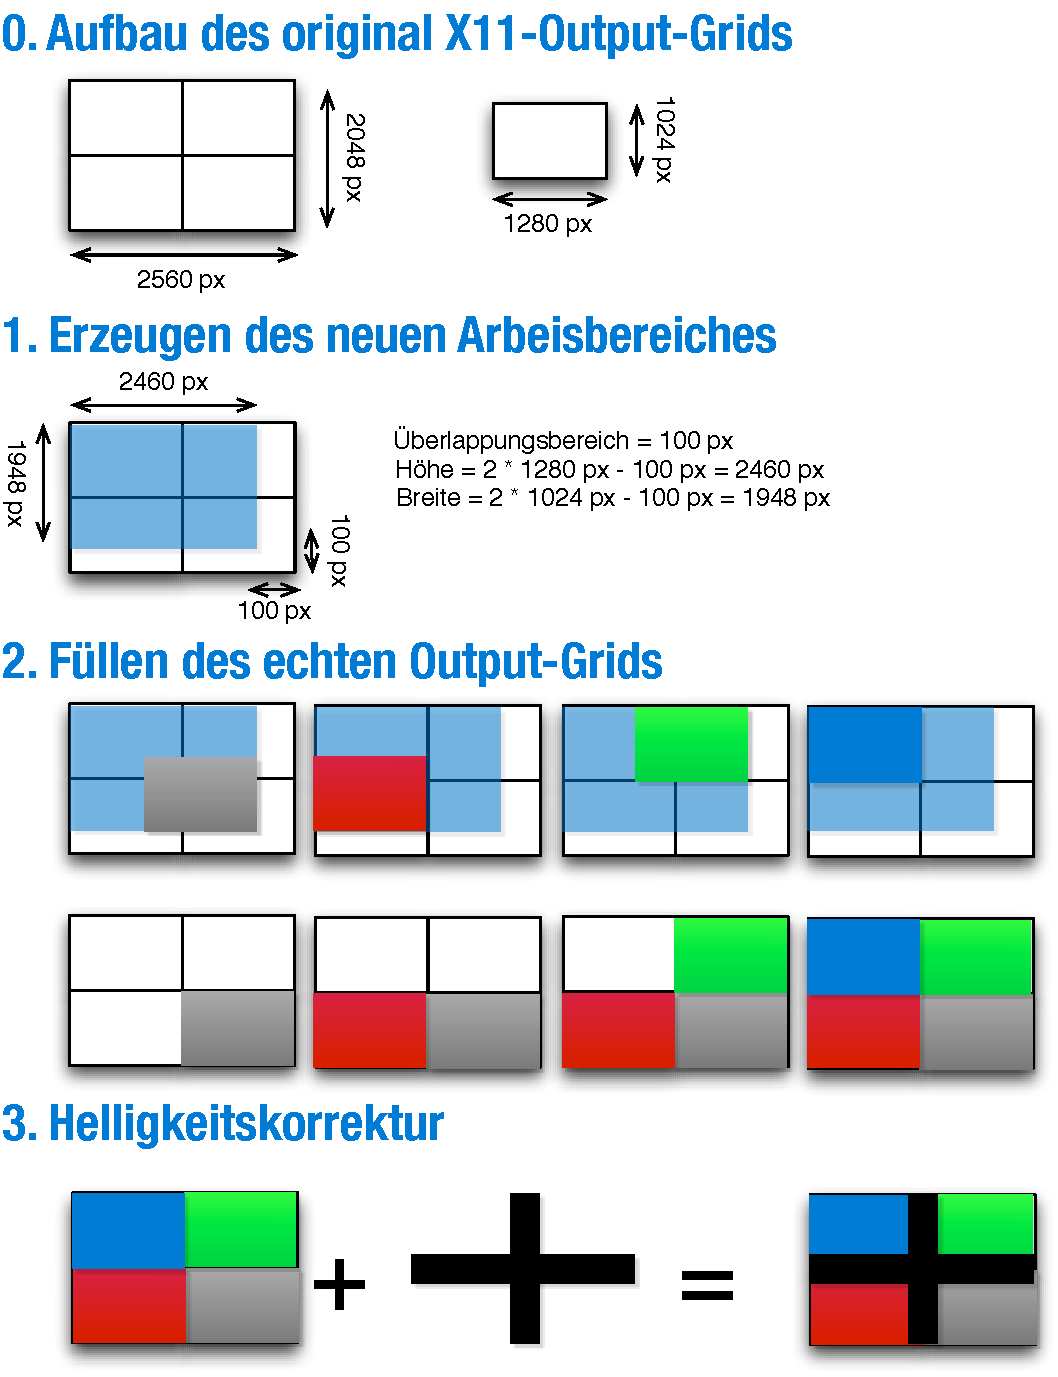
\includegraphics[width=\linewidth]{gfx/outputerzeugung.pdf}
\caption{Erzeugung des Egeblendings}
\label{fig:gridoutput}
\end{figure}
\newpage

\subsection{Generieren der Blending-Maske}
Nachdem im vorherigen Abschnitt beschrieben wurde, wie die erzeugte Maske mit der eigentlichen Benutzeroberfl�che zusammengef�gt wird, beschreibt dieser Abschnitt wie die Maske erstellt wird.
Resultierend muss die Maske als Grafik vorliegen, die �ber jeden Output geblendet werden kann. Daher muss entweder pro Ausgabeger�t eine Maske erzeugt werden oder eine die �ber alle Ausgaben angewendet werden kann. Die Konfiguration l�sst hier f�r den Blending-Verlauf pro Seite eines Screens eine Funktion 2. Grades zu. Dies sind die Restriktionen, die f�r das Generieren der Maske gelten.

\subsubsection{Analyse}
Die beiden M�glichkeiten zur Generierung der Maske sind �ber
\begin{enumerate}
  \item absolute Funktionen und Relationen oder
  \item relative Funktionen m�glich.
\end{enumerate}

Absolute Funktionen f�r die obere und untere Kante, sowie Relationen f�r die linke und rechte Kante des Screens sind unpraktikabel, da nicht davon ausgegangen werden kann, dass es immer eindeutige links-rechts, oben-unten zuordnungen gibt. Zudem ist es f�r den konfigurierenden Benutzer nicht so einfach die gew�nschten Funktionen und Relationen zu erstellen wie in der zweiten M�glichkeit.

Die Funktionen relativ zur jeweiligen Seite zu erstellen, mit der Seite als X-Koordinate und dem linken Ende als Nullpunkt ist wesentlich intuitiver.

Eine zus�tzliche unabh�ngige M�glichkeit kann dadurch gegeben werden, dass ein Bild eingelesen wird welches beliebig durch ein Grafikbearbeitungsprogramm manipuliert werden kann.


\subsubsection{Realisation}
Gew�hlt wurde der intuitivere Ansatz der relativen Funktionen und die unabh�ngige M�glichkeit die Maske direkt vorzugeben. So wird jede Seite jedes Screen die jeweilige Funktion aus der Konfiguration entnommen. Die Errechnung des Blending-Wertes geschieht durch vertauschen der Koordinaten, so dass das linke Ende einer Seite den Nullpunkt im Koordinatensystem darstellt. Es lassen sich mit einigen Additionen und Subtraktionen die Funktionen auf die vier Seiten eines Screens abbilden.

F�r die Manipulation der Helligkeit muss einzig der Alpha-Wert angepasst werden. Die anderen drei Werte werden nicht angepasst. Bei der Anpassung wird dabei pro Pixel errechnet ob dieser unterhalb einer Funktion liegt und dem entsprechend wird Anteilig zwischen dem Au�enrand des Screen und der Funktion der Alpha-Wert gesetzt. An den Ecken m�ssen diese Werte nat�rlich verrechnet werden, wenn der betreffende Pixel unterhalb zweier Funktionen liegt.

Wenn $f$ die Blendingfunktion und $p$ der aktuell betrachtete Pixel ist. $a$, $b$ und $c$ $f$ als $f(x) = a*x^2 + b*x + c$ definieren und $p_y < f(p_x)$ ist, dann ist $p_alpha = (f(p_x) - p_y) / f(p_x)$ (nat�rlich nur f�r $f(p_x) > 0$).

Da die Bilddaten auf Wunsch direkt abgelegt werden k�nnen, sind diese auch f�r exotischere Projektionsoberfl�chen manipulierbar. Obwohl mit einer Funktion 2. Grades pro Screen-Kante selbst Edgeblending bei Halbkugeln kein Problem ist.
Wenn die Maske nicht aus der Datei gelesen wird dauert das Starten des Plug-In l�nger, da sie komplett erstellt werden muss.
  %%%%%%%%%%%%%%%%%%%%%%%%%%%%%%%%%%%%%%%%%%%%%%%%%%%%%%%%%%%%%%%%%%%%%%%
\section{Beschreibung grundlegender Datenstrukturen}
\label{sec:programmierhandbuch:datenstrukturen}

%Hier werden die Datenorganisation und die Datenstrukturen zur Probleml�sung beschrieben. Dazu z�hlt der Aufbau, die Gr��e der einzelnen Komponenten und speziell bei dynamischen Strukturen die Verzeigerung untereinander. In diesem Zusammenhang ist auch der Aufbau der vom Programm benutzten Datendateien zu beschreiben.
\subsection{Konfigurationsdatei und deren interne Repr�sentation}

F�r die Beschreibung der XML-Dateistruktur siehe Sektion \ref{sec:benutzerhandbuch:anleitung}. Intern wird ebendiese Struktur �bernommen.

\mylisting[label=lst:output, caption={Interne Darstellung der Konfiguration}]{listings/output.h}

\subsection{Formatierung der Bilddateien}
Die Bilddateien, die optional in der Konfigurationsdatei angegeben werden k�nnen sind "`TGA"' Dateien (Truevision Graphics Adapter). Auch bezeichnet als "`TARGA"'. Die Bilddateien m�ssen um korrekt gelesen zu werden unkomprimierte Daten ohne Farbtabelle enthalten. Dabei werden vier Byte pro Pixel abgelegt, je ein Byte f�r rot, gr�n, blau und alpha Darstellung. Wesentlich ist aktuell nur der Alpha-Wert, der beschreibt wie stark der jeweilige Ausgabebereich abgedunkelt wird.
  %%%%%%%%%%%%%%%%%%%%%%%%%%%%%%%%%%%%%%%%%%%%%%%%%%%%%%%%%%%%%%%%%%%%%%%
\section{Programmorganisation}
\label{sec:programmierhandbuch:organisation}

Ein Programmorganisationsplan (POP) gibt die Aufrufhierarchie aller Unterprogramme eines Programms wieder. Noch besser als ein einfacher POP ist eine Darstellung in Form von Structure-Charts.

\todo{diese sektion {\it hat keinen sinn???? }}
  %%%%%%%%%%%%%%%%%%%%%%%%%%%%%%%%%%%%%%%%%%%%%%%%%%%%%%%%%%%%%%%%%%%%%%%
\section{Programmtest}
\label{sec:programmierhandbuch:test}

Zur Beschreibung eines Programmtests geh�rt eine Auflistung der Testeingabedaten, der erwarteten und der errechneten Ergebnisdaten. Bei Abweichungen sind Begr�ndungen anzugeben und das Programm entsprechend zu beurteilen (z.B. "Eine Ungenauigkeit von 0.005 \% ergibt sich aus dem numerischen Darstellungsbereich des Datentyps XYZ und ist f�r die erwarteten Werte vertretbar."). Grundlage der Auswahl der Testdaten ist der White Box-Test, der gew�hrleistet, da� alle Programmteile durchlaufen werden. Die Auswahl der verwendeten Testdaten ist zu begr�nden, z.B. Indexwerte 99, 100 und 101, um bei einem Array von 100 Werten die Grenz�berschreitung zu pr�fen.

%\appendix

% \backmatter
%\bibliographystyle{alphadin}
\label{app:bibliography} 
\bibliography{bibliography/bibliography,bibliography/rfc,bibliography/w3c}
%%%%%%%%%%%%%%%%%%%%%%%%%%%%%%%%%%%%%%%%%%%%%%%%%%%%%%%%%%%%%%%%%%%%%%%%%%%%%%%%%
% Affidavit
%%%%%%%%%%%%%%%%%%%%%%%%%%%%%%%%%%%%%%%%%%%%%%%%%%%%%%%%%%%%%%%%%%%%%%%%%%%%%%%%
\addchap{Affidavit}
\label{cha:aff}
I hereby declare that this thesis has been written independently by me, solely based on the specified literature and resources. All ideas that have been adopted directly or indirectly from other works are denoted appropriately. This thesis has not been submitted to any other board of examiners in its present or a similar form and was not yet published in any other way.

\bigskip

Wedel, \Datum

\vspace{5ex}

\begin{center}
(\Author)
\end{center}

\end{document}